\documentclass{sig-alternate}
%\documentclass[a4paper,10pt]{article}
\usepackage[utf8]{inputenc}
%El template pincha con spanish babel
%\usepackage[spanish]{babel}
\usepackage{graphicx}
\usepackage{fancybox}
\usepackage[table]{xcolor}
\usepackage{soul}

\title{Banzai Totsugeki} 

\numberofauthors{4}
\author{
\alignauthor
Pose, Alberto Miguel\\
       \affaddr{ITBA}\\
       \affaddr{Madero 399}\\
       \affaddr{Buenos Aires, Argentina}\\
       \email{apose@alu.itba.edu.ar}
\alignauthor
Catalano, Juan Ignacio\\
       \affaddr{ITBA}\\
       \affaddr{Madero 399}\\
       \affaddr{Buenos Aires, Argentina}\\
       \email{jcatalan@alu.itba.edu.ar}
\and
\alignauthor 
Palombo, Martín\\
       \affaddr{ITBA}\\
       \affaddr{Madero 399}\\
       \affaddr{Buenos Aires, Argentina}\\
       \email{mpalombo@alu.itba.edu.ar}
\alignauthor 
Vázquez, Santiago Luis\\
       \affaddr{ITBA}\\
       \affaddr{Madero 399}\\
       \affaddr{Buenos Aires, Argentina}\\
       \email{savazque@alu.itba.edu.ar}
}

%Viejo author
%\author{Catalano, Juan Ignacio \crcr Palombo, Martín \crcr Pose, Alberto Miguel \crcr Vázquez, Santiago Luis}

\date{}

\begin{document}

\maketitle

\begin{abstract}
\hl{En el presente art\'iculo se modela un combate guerra-guerra, considerando las fuerzas como medida del poder\'io de ambas partes y 
analizando el modelo constru\'ido para obtener conclusiones mediante su observaci\'on. De dicho an\'alisis se desprende que el uso del modelo planteado
resulta adecuado para simular esta batalla, obteniendose resultados similares a los sucedidos. Tambi\'en se analiza el comportamiento del sistema,
mediante la observaci\'on del modelo, variando las funciones de refuerzos enviados a la batalla. Adem\'as se realiza una deducci\'on anal\'itica que
concluye en una interesante descripci\'on de la relaci\'on de efectividad de combate entre ambas fuerzas. CAMBIAR}
\end{abstract} 



\newpage

\section{Introducci\'on}

El 16 de febrero de 1945, durante la segunda guerra mundial, se libra la batalla de Iwo Jima en la isla de nombre homónimo. 
Siend sin duda uno de los acontecimientos bélicos más sangrientos y lamentables de la historia. La ubicación geográfica estratégica de dicha
isla otorga gran importancia histórica a esta batalla y es por ello que nos interesa nos interesa estudiarla como un sistema, modelándola y 
pudiendo extraer conclusiones a partir de dicho modelo. Se pretende verificar el modelo utilizado,
computando y analizando los resultados obtenidos de la simulación y variando parámetros del mismo. Se pueden encontrar antecedentes a este 
trabajo, como por ejemplo el llevado acabo por Christine Lind titulado ``Verifying Lanchester’s Combat Model Battle of Iwo Jima''. \\ 
En la siguiente secci\'on se presenta el modelo utilizado para realizar dicha simulaci\'on. En la tercer secci\'on se adapta el modelo genérico,
previamente mostrado, al caso particular de la batalla de Iwo Jima. En la sección cuatro se presenta un resultado matem\'atico-f\'isico cuya 
importancia se explica en la misma secci\'on. En la secci\'on cinco se presentan los resultados obtenidos a partir de la simulaci\'on. En la
sexta sección se modela nuevamente la batalla pero utilizando distintas funciones de refuerzo para las fuerzas militares estadounidenses.
Por \'ultimo, en la secci\'on siete se agrupan las conclusiones obtenidas durante la realizaci\'on del trabajo.

\section{``La mejor victoria es vencer sin combatir''}
Para modelar este sistema se consideran las dos fuerzas militares representadas por ($x^1(t), x^2(t)$) siendo la primera correspondiente a Estados
Unidos y la segunda al Imperio de Japón. La medida de estas variables representa el poderío de ambas partes del combate. 
El vector definido como:

\begin{equation}
x(t) = ( x^1(t), x^2(t) )^T \label{eq:state_vector}
\end{equation}

representa el vector de estado, es decir, el poderío de ambas partes en el instante $t$. El espacio de estados se considera como la cantidad de 
unidades de combate, considerando todo tipo de ellas (individuos, equipos, recursos, etc). Como es de esperarse, las entradas al sistema estan 
dadas por los refuerzos enviados por cada uno de los países.\\
Hasta aquí, la representación del modelo de combate. Pero en particular, nos referimos a un combate de tipo guerra-guerra, es decir, convencional.
En este caso, las pérdidas en combate están solamenten dadas por el tamaño de la fuerza contraria, con lo cual nuestro modelo queda descripto de la
siguiente manera:

\begin{equation}
\dot{x}^1(t) = -ax^1(t) - c_{21} x^2(t)\end{equation}
\begin{equation}
\dot{x}^2(t) = -bx^2(t) - c_{12} x^1(t)\end{equation}

Siendo $a$ y $b$ constantes positivas que representan las tasas unitarias de pérdidas operativas. Teniendo también $c_{12}, c_{21}$ 
constantes positivas que representan las tasas de efectividad de ataque de la fuerza 1 sobre la 2 y de la fuerza 2 sobre la 1 respectivamente.

\section{Recordando la historia}

En esta sección se utiliza una adaptación del modelo presentado anteriormente para simular el sistema dado por el combate entre Japón y 
Estados Unidos de América, en la ciudad de Iwo Jima en febrero de 1945. Inicialmente Japón cuenta con una fuerza de 21500 unidades 
atrincheradas en el lugar, mientras que su enemigo incialmente no dispone de unidades en Iwo Jima y envía refuerzos siguiendo el siguiente 
régimen:

\begin{equation}
f(t) = \left\{ 
    \begin{array}{l l}
    54000 & \quad 0 \leq t < 1 \\
    0 & \quad 1 \leq t < 2\\
    6000 & \quad 2 \leq t < 3\\
    0 & \quad 3 \leq t < 5\\
    13000 & \quad 5 \leq t < 6\\
    0 & \quad t \geq 6\\
    \end{array} \right.
\end{equation}
Siendo $f$ la función que describe la llegada de refuerzos de los Estados Unidos. Como se considera que Japón no envía refuerzos durante este
combate, el modelo resulta descripto por:


\begin{eqnarray}
\dot{x}^1 &=& -\alpha x^2 + f(t)                              \\
\dot{x}^2 &=& -\beta x^1
\end{eqnarray}


\section{Poder K}

A partir de un modelo sin refuerzos y realizando una integración analítica obtenemos una relación entre las fuerzas de combate y una constante (constante de integración):

Tenemos

\begin{eqnarray}
\dot{x} & = & -\alpha y\label{eq:ydot}\\
\dot{y} & = & -\beta x\end{eqnarray}


Explicitando, obtenemos la expresión

\begin{equation}
\dot{x}=-\alpha y\end{equation}


Como sabemos que $\dot{x}=\frac{d x}{d y}\frac{d y}{d t}$:

\begin{equation}
\frac{d x}{d y}\dot{y}=\frac{d x}{d y}\frac{d y}{d t}=-\alpha y\end{equation}


Reemplazando con la ecuación \eqref{eq:ydot} resulta

\begin{equation}
-\frac{d x}{d y}\beta x=-\alpha y\end{equation}


Reemplazando adecuadamente los diferenciales tenemos 

\begin{equation}
-\beta\intop x dx + C =-\alpha\int y dy + D\end{equation}


Siendo $C$ y $D$ constantes de integración. Podemos considerar $D - C = k$. De lo cual deducimos

\begin{equation}
\alpha\frac{y^{2}}{2}-\beta\frac{x^{2}}{2}=k\end{equation}


Considerando $K=2k$ se puede reescribir de la siguiente manera:

\begin{equation}
\alpha y^{2}-\beta x^{2}=K\label{eq:obtenida}\end{equation}

Si fijamos los parámetros del sistema $\alpha$ y $\beta$ se obtiene una relación entre ambas fuerzas de combate. Esta ecuación representa una familia de hip\'erbolas cuando $K \ne 0$. Mientras que en el caso de $K = 0$ se obtiene la recta asíntota.
\begin{figure}[h]
\begin{center}
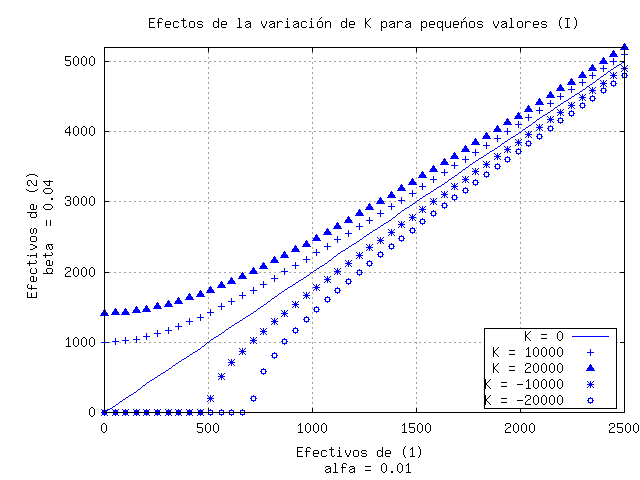
\includegraphics[width=8cm]{power_areas_1}
\caption{\label{fig:powerarea1} Gr\'afico obtenido de fijar $\alpha = 0.01$ y $\beta = 0.04$ en la ecuación \ref{eq:obtenida}. Se muestra el comportamiento del sistema sin políticas de refuerzos para distintos K.}
\end{center}
\end{figure}
\begin{figure}[h]
\begin{center}
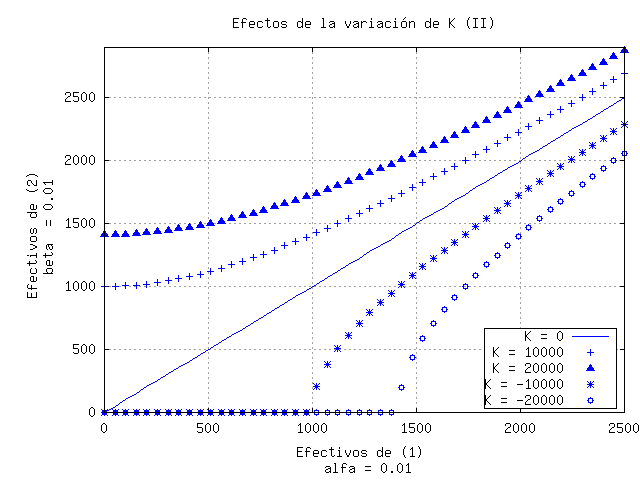
\includegraphics[width=8cm]{power_areas_2}
\caption{\label{fig:powerarea2} Gr\'afico obtenido de fijar $\alpha = 0.01$ y $\beta = 0.04$ en la ecuación \ref{eq:obtenida}. Se muestra el comportamiento del sistema sin políticas de refuerzos para distintos K.}
\end{center}
\end{figure}


El an\'alisis s\'olo tiene sentido cuando la cantidad de unidades son positivas. Por lo tanto, limitaremos el an\'alisis al primer cuadrante del plano cartesiano como puede observarse en \ref{fig:powerarea1} y \ref{fig:powerarea2}:


\textbf{\textit{Caso 1.}} En el caso donde $K > 0$ corresponden a hip\'erbolas que comienzan
sobre el eje de las ordenadas. En este caso quiere decir que la fuerza representada
en el eje Y ganar\'ia el combate de no aumentarse la cantidad de tropas
el contricante.


\textbf{\textit{Caso 2.}} Si $K<0$ se tienen hip\'erbolas que comienzan
en el eje de las abcisas. Esto es igual que el caso anterior pero resultando vencedor el ejército del eje x.

\textbf{\textit{Caso 3.}} 
En $K=0$ la relación entre los ejércitos describe una recta. Dado los parámetros del sistema $\alpha$ y $\beta$ podemos encontrar la pendiente como $\sqrt{\frac{\beta}{\alpha}}$. Dicha recta determina el grado de efectividad de las unidades militares de una fuerza sobre la otra. Una vez fijada la pendiente, se puede 
establecer qué cantidad de unidades son necesarias de una fuerza, ante la presencia de determinada cantidad de unidades enemigas.  \\
La interpretación f\'isica ser\'ia un combate balanceado. no quiere decir que se tiene la misma cantidad de efectivos desplegados. Sino que el poderío militar de los dos ej\'ercitos está equilibrado en función de $alpha$ y $beta$. Es decir, que en caso de no contar con una funci\'on de refuerzo se terminar\'ia con cero efectivos de ambos lados. \\
Volviendo al caso $K \ne 0$, cuanto m\'as cerca est\'en de la as\'intota las hip\'erbolas son m\'as desgastantes para el ejercito. Esto es decir que aunque sea claramente
el vencedor el lado en el que se encuentra la hip\'erbola, el costo
podr\'ia ser muy alto. En cambio cuando se está lejos de la as\'intota
quiere decir que se está ganado sin tantas bajas. \\

La función de refuerzo juega un rol importante en la batalla. Permite la modificación del K que describe la hipérbola donde transcurre la batalla. Esto permite:
\begin{enumerate}
\item reducir las bajas al alejarse de la recta asíntótica $K=0$
\item modificar el resultado de una batalla en caso de
\end{enumerate}


\section{Reviviendo la historia}

Para poder realizar un análisis de lo acontecido en la batalla, se ejecutó la simulación para obtener las 
trayectorias correspondientes a ambas fuerzas. En la figura \ref{fig:trays} se pueden ver dichas trayectorias. 
De este podemos observar como, si bien inicialmente las fuerzas militares del Japón eran ampliamente superiores, el hecho de no disponer de 
refuerzos, como en el caso estadounidense, llevó a una rápida extinción del poderío militar presente en la zona. Por parte de los 
Estados Unidos, se vé como si bien su fuerza fue decreyendo a un ritmo similar a la japonesa, la mayor presencia militar llevó a que finalmente
se note una clara preponderancia de este país en el conflicto. También podemos observar un decaimiento lineal en el caso de las fuerzas japonesas,
en contraparte con uno más exponencial (aunque bastante suavizado) por parte de las estadounidenses.\\
Además, podemos verificar el uso del modelo elegido para la simulación. Para ello, comparamos los resultados obtenidos con los datos 
recolectados a partir del hecho acontecido. Dicha comparación, correspondiente a la fuerza estadounidense, la graficamos en la figura 
\ref{fig:realvssim}.
Podemos observar el desembarco, en la primer etapa, donde vemos claramente como aumenta rápidamente la cantidad de unidades. A su vez, durante los primeros 5 días al recibirse los refuerzos, se
puede ver como se producen picos, donde los aumentos estan dados por la llegada de nuevas unidades y las disminuciones más bruscas estan dadas
por las bajas producidas durante el asentamiento de las tropas en el área de batalla.\\
Otra gráfica realizada es la Figura \ref{fig:xvsy} en donde proyectamos la simulación, graficando las fuerzas militares
estadounidenses, en funcion de las japonesas. Como se puede ver, observando el gráfico aproximadamente en el punto $20000$ de las ordenadas,
encontramos que las fuerzas estadounidenses son cero. Este es el comienzo de la batalla. Luego, podemos ver como con la llegada de refuerzos 
estadounidenses se va decrementando la cantidad de efectivos japoneses. Además, se puede observar como la función que representa la cantidad de
efectivos americanos se aproxima a una de las hipérbolas descriptas en la sección anterior. Esto ocurre a medida que se envían los refuerzos,
para culminar en el momento donde ya no hay más envíos. La elección de la constante $K$ fue determinada de forma empírica.

\begin{figure}[h]
\begin{center}
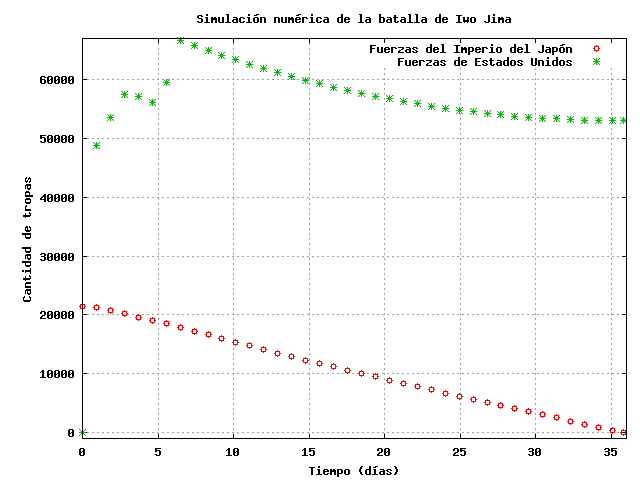
\includegraphics[width=8cm]{jap_vs_usa.png}
\caption{\label{fig:trays}Cantidad de tropas de ambas fuerzas en función del tiempo.}
\end{center}
\end{figure}

\begin{figure}[h]
\begin{center}
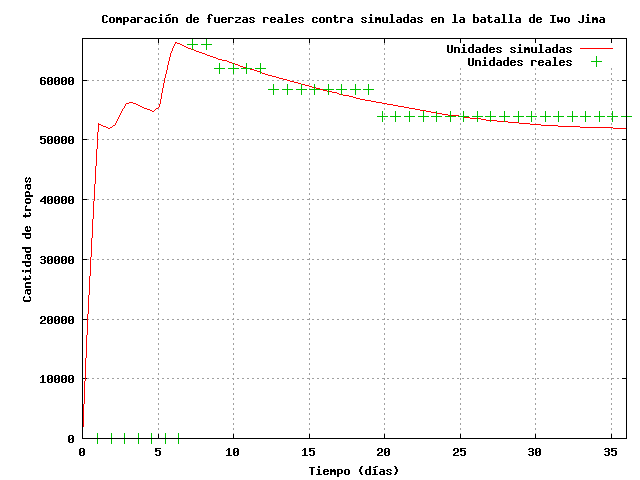
\includegraphics[width=8cm]{real_vs_sim.png}
\caption{\label{fig:realvssim}Cantidad de tropas estadounidenses en función del tiempo. Datos correspondientes al hecho y a la simulación.}
\end{center}
\end{figure}

\begin{figure}[h]
\begin{center}
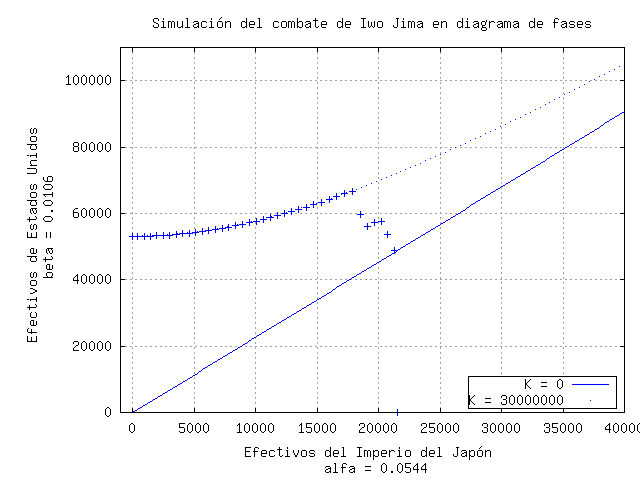
\includegraphics[width=8cm]{power_area_iwo_jima.png}
\caption{\label{fig:xvsy}Cantidad de tropas estadounidenses en función de las japonesas.}
\end{center}
\end{figure}

\newpage

\section{Haciendo historia}

¿Qué hubiese sucedido si la política de envío de refuerzos de Estados Unidos hubiese sido distinta?. Para responder esta pregunta, veamos como
reacciona el sistema al cambiar las políticas de envio de refuerzos estadounidenses.\\
Se eligieron las tres políticas analizadas en base a la observación de su comportamiento y seleccionando las que nos arrojaron resultados
más interesantes para su análisis. Dichas políticas, que denominamos $g$, $h$ y $k$ las podemos observar en las ecuaciones \eqref{eq:refuerzo_g}, 
\eqref{eq:refuerzo_h} y \eqref{eq:refuerzo_k} respectivamente.

\begin{equation}
g(t) = \left\{ 
    \begin{array}{l l}
    30000 & \quad 0 \leq t < 1 \\
    0 & \quad 1 \leq t < 4\\
    3000 & \quad 4 \leq t < 5\\
    0 & \quad 5 \leq t < 7\\
    1000 & \quad 7 \leq t < 8\\
    0 & \quad t \geq 8\\
    \end{array} \right.
\label{eq:refuerzo_g}
\end{equation}

\begin{equation}
h(t) = \left\{ 
    \begin{array}{ll}
    54000 - \lfloor 9000t \rfloor & \quad 0 \leq t \leq 6 \\
    0 & \quad t > 6\\
    \end{array} \right.
\label{eq:refuerzo_h}
\end{equation}

\begin{equation}
k(t) = \left\{ 
    \begin{array}{l l}
    54000 & \quad 0 \leq t < 1 \\
    0 & \quad 1 \leq t < 20\\
    6000 & \quad 20 \leq t < 21\\
    0 & \quad 21 \leq t < 35\\
    13000 & \quad 35 \leq t < 36\\
    0 & \quad t \geq 36\\
    \end{array} \right.
\label{eq:refuerzo_k}
\end{equation}


Notamos que la política de refuerzo $k$ es una variación de la política original, pero extendiendo la cantidad de días entre refuerzos.
Si observamos la gráfica presentada en la figura \ref{fig:reinforce2} podemos ver que esta política resulta en un comportamiento del sistema
que equipara la cantidad de unidades de una y otra fuerza en cierto punto del tiempo $t$.\\
Si vemos el resultado de la simulación para la política de refuerzo $g$, podemos observar que dado este escenario, el ejército estadounidense es derrotado por el japonés. Podemos 
concluir que si EEUU hubiese este acercamiento, posiblemente el resultado hubiese sido distinto impactando fuertemente en el desarrollo de la Segunda Guerra Mundial.\\
Por otro lado, si vemos el comportamiento del sistema al elegir $h$ como política de refuerzos, presentado en la figura \ref{fig:reinforce3}, 
podemos ver como la preponderancia de las tropas estadounidenses aumenta y supera ampliamente a la japonesa de una manera mucho más conveniente que la elegida originalmente.\\
Finalmente, analizamos la política de refuerzo $k$; siendo ésta una variación a la política original. Si observamos el resultado del combate en la figura \ref{fig:reinforce4}
vemos que ambas fuerzas decrecen de una manera aproximadamente lineal en el tiempo(en el caso de EEUU, hasta que recibe refuerzos). Lo interesante es que la pendiente de la recta
que modela las fuerzas estadounidenses es mucho más abrupta que la japonsa. Ésto implica que el ejército japonés era más eficiente en batalla y sirve para destacar lo
importante del papel que juegan las constantes PONELE NOMBRE SON C12 C21 O ALFA BETA SER CONSISTENTEEES. Mediante el resultado de la siumulación podemos apreciar
que los japoneses realmente lucharon hasta el final.

\begin{figure}[h]
\begin{center}
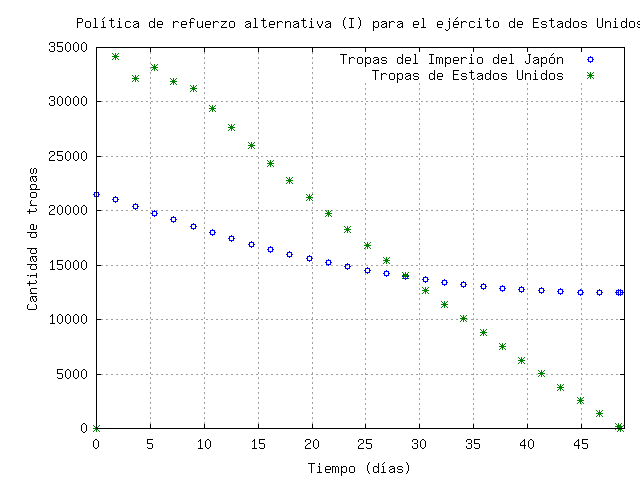
\includegraphics[width=8cm]{reinforce2.png}
\caption{\label{fig:reinforce2}Resultados del combate simulado usando la política de refuerzos alternativa $h$.}
\end{center}
\end{figure}

\begin{figure}[h]
\begin{center}
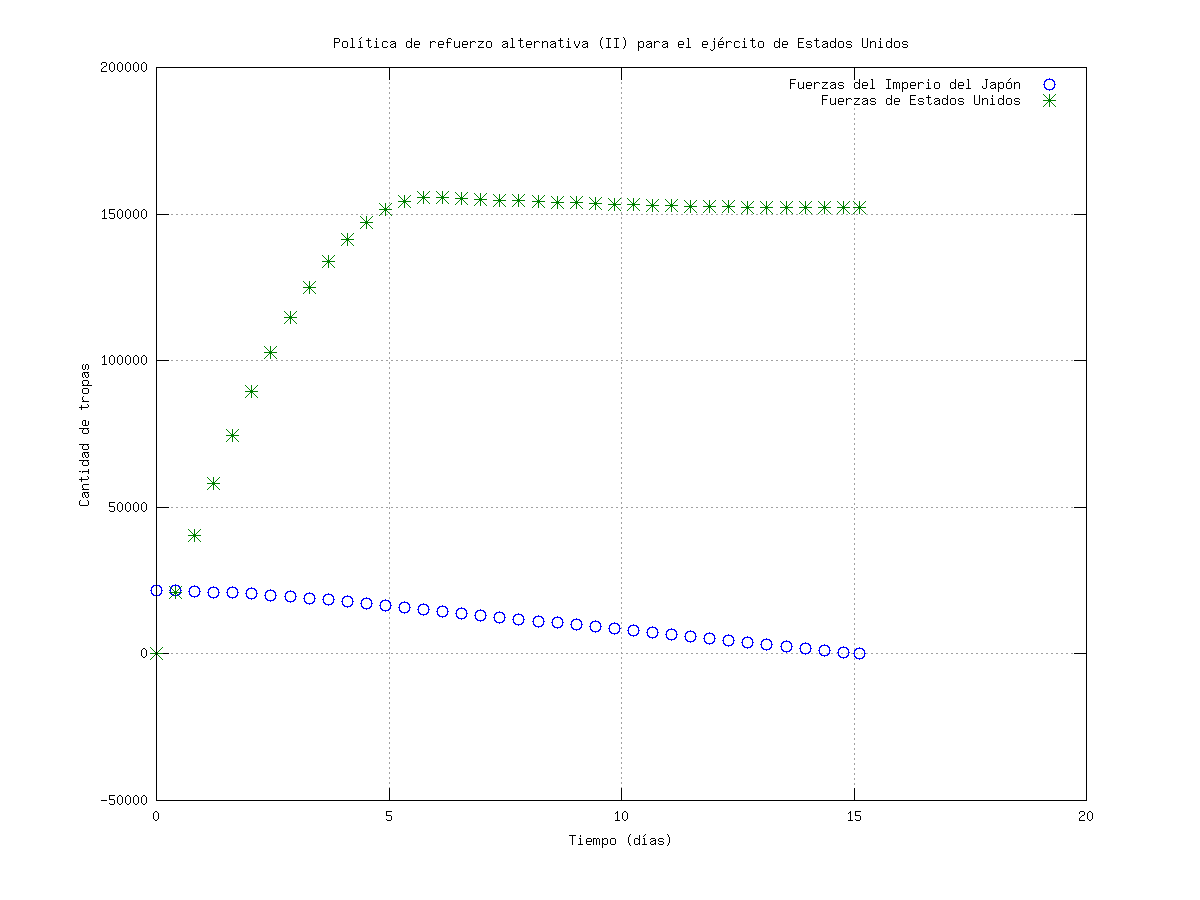
\includegraphics[width=8cm]{reinforce3.png}
\caption{\label{fig:reinforce3}Resultados del combate simulado usando la política de refuerzos alternativa $g$.}
\end{center}
\end{figure}


\begin{figure}[h]
\begin{center}
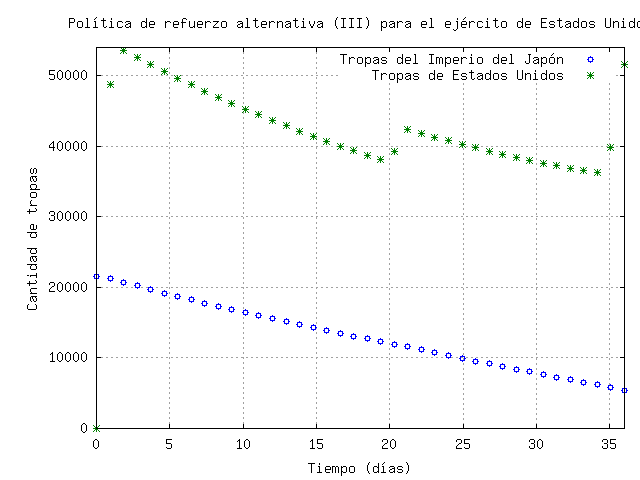
\includegraphics[clip, width=8cm]{reinforce4.png}
\caption{\label{fig:reinforce4}Resultados del combate simulado usando la política de refuerzos alternativa $k$.}
\end{center}
\end{figure}


\section{Conclusiones y Resultados}
\subsection{Política de refuerzos}



Al realizar este trabajo se pudo verificar el modelo elegido, analizando los resultados para compararlos con los datos recolectados historicamente
a partir del hecho acontecido. Como conclusión a los cambios de política de refuerzos realizados, se puede decir que EEUU podría haber considerado una
mejor política de refuerzos, aunque requeriría un análisis socio-económico y político más profundo para poder determinar porque realmente no
lo hizo.\\
Puntos interesantes que se pueden observar de la primer simulación realizada, son los picos obtenidos al momento de la llegada de refuerzos
estadounidenses y las pérdidas iniciales durante la etapa de asentamiento, que se ven claramente en las irregularidades iniciales de la curva 
graficada.\\
Otra conclusión importante es la relación obtenida entre las fuerzas en combate. Particularmente, resaltar que ante una relación lineal de las
fuerzas, es decir, el caso en el que la constante $K$ es igual a $0$, la recta descripta nos proporciona bases de trabajo para estimar estadísticas \\
La política de refuerzos permite variar el $K$ que describe la
hip\'erbola que representa el combate, de manera de alterar el
resultado. Podr\'ia pensarse el sistema sin refuerzos como a lazo
abierto: el resultado del combate está \'unicamente determinado
por la cantidad de tropas y las tazas de efectividades. Por otra
parte, a lazo cerrado ser\'ia utilizando la funci\'on de refuerzos de
manera de alterar el combate para que un lado sea el vencedor en menor
cantidad de tiempo o sacrificando menos unidades. Un análisis interesante, aunque escapa al trabajo, sería tener dos funciones de refuerzos (una por cada ejército). \\
El mayor inconveniente para lograr esto es la complicación de establecer a priori tanto $\alpha$ como $\beta$.
como la efectividad de las unidades militares de cada fuerza, contra las enemigas.

\end{document}
